\documentclass[10pt,a4paper,twocolumn]{article}

\usepackage[T2A]{fontenc}
\usepackage[utf8]{inputenc}

\usepackage[backend=biber]{biblatex}
\addbibresource{ref.bib}

\usepackage{amsmath}
\usepackage{amssymb}
\usepackage{commath}
\usepackage{titlesec}
\usepackage{graphicx}
\usepackage{caption}
\usepackage{subcaption}
\usepackage{indentfirst}
\usepackage{hyperref}
\usepackage{enumitem}[leftmargin=0pt]
\usepackage{verbatim}
\usepackage{bm}
\usepackage{float}

\renewcommand{\vec}[1]{\bm{\mathrm{#1}}}

\begin{document}

\title{Hail}
\author{\today}
\date{}
\maketitle

\clearpage

\section{Problem statement}

Extract as much information as possible about the shape and dimensions of a metal container from the sound produced when dropping small objects (such as peas) into it.


\section{Introduction}

The question of whether we can "hear the shape of a drum" has been researched extensively.\cite{mathans} \cite{kac} The heart of the problem lies in the eigenfrequencies of oscillation of the object, because other properties of the sound are too dependent on external factors to be used to reliably reconstruct the shape of the oscillating body. Mathematically, the question becomes "Can the eigenvalue spectrum of the Laplace operator uniquely determine the geometry of the domain and boundary on which it is defined?". The answer to this question has been found and is no in full generality, but counterexamples are usually contrived. The exactness of the mathematical question is physically muddled by the fact that open ends aren't exactly modeled as Neumann boundary conditions, requiring further end corrections.

We first focus on solving the inverse question, namely finding the eigenfrequencies analytically for common simple geometries in 3D and additionally comment on other solutions for the sides and other more complicated shapes. We further discuss the experimental limitations that arise and limit the information we are able to extract and the results we obtained from experiments.


\section{Theoretical description}

To better understand the question of reverse engineering the shape and size of an object from its sound we should first look at the inverse problem -- finding the resonant frequencies of the object.

The answer to this question amounts to finding standing wave solutions of the wave equation
%
\begin{align}
\nabla^2 \Psi(\vec{r}, t) - \frac{1}{c^2} \frac{\partial \Psi(\vec{r}, t)}{\partial t} = 0
\end{align}
%
with a Dirichlet boundary condition for closed ends and a Neumann boundary condition for open ends, where $c$ is the speed of sound in the material.

Separating variables as $\Psi(\vec{r}, t) = \psi(\vec{r}) f(t)$ reveals that this is just the problem of finding the spectrum of the Laplacian operator
%
\begin{align}
\nabla^2 \psi(\vec{r}) = -k^2 \psi(\vec{r})
\end{align}
%
where $k^2$ is a separation constant that we recognize as the wavenumber. The boundary conditions give us limitations on this wavenumber which, in turn, lead to the resonance peaks in the spectrum through
%
\begin{align}
\nu = \frac{c}{2 \pi} k
\end{align}

We now look at the two special cases of a rectangular and a cylindrical geometry.

\subsection{Rectangular geometry}

In this case the solutions are found by further  separating every Cartesian direction. For the volumetric resonances the boundary conditions are Dirichlet for all but one of the sides if the container is open and they are Dirichlet for all sides if the container is closed leading to the eigenfrequencies
%
\begin{align}
\nu = \frac{c}{2} \sqrt{\left(\frac{n}{L_x}\right)^2 + \left(\frac{m}{L_y}\right)^2 + \left(\frac{l}{L_z}\right)^2}
\end{align}
%
where $L_x$, $L_y$ and $L_z$ are the side lengths, $n, m \in \mathbb{N}_0$, $l \in \mathbb{N}_0$ if the container is closed and $l \in \mathbb{N}/2$ if the container is open.

\subsection{Cylindrical geometry}

For this case it's obviously convenient to work in cylindrical coordinates where the Laplacian takes the form
%
\begin{align}
\nabla^2 = \frac{1}{r} \frac{\partial}{\partial r}\left(r \frac{\partial}{\partial r}\right) + \frac{1}{r^2} \frac{\partial^2}{\partial \phi^2} + \frac{\partial^2}{\partial z^2}
\end{align}
%
Separating variables, this time as $\psi(r, \phi, z) = R(r) \Phi(\phi) Z(z)$, gives us the usual sinusoids $\sin$ and $\cos$ as solution for the $Z$ and $\Phi$ functions and Bessel functions as solutions for the radial part $R$. Imposing the condition of regularity at the origin removes the Bessel $Y_m$ function as a possible solution. The further conditions of $R(a) = 0$ at the radial boundary and the usual open-closed conditions on $Z$ for the vertical boundaries we get the requirement for resonance
%
\begin{align}
\nu = \frac{c}{2} \sqrt{\left(\frac{\rho_{m,n}}{\pi a}\right)^2 + \left(\frac{l}{H}\right)^2}
\end{align}
%
where $a$ is the radius, $H$ is the height and $\rho_{m,n}$ is the $n$-th zero of the $m$-th Bessel $J_m$ function. The number $l$ is the same as in the rectangular case, namely with the same dependence on the container being open/closed.

\subsection{Other solutions}

The complications of other solutions come in two forms.

Firstly, in 3D, it's not possible to solve the equations analytically for many other geometries, and those for which we can aren't usually used as containers, meaning an experiment can't be done to confirm or deny our calculations.

Secondly, the sides simply can't be approximated as just 2D membranes. We have to describe them, at least, as Kirchhoff-Love isotropic plates.\cite{kirchhoff} \cite{love} These equations, although solvable in the case of simple geometries for isotropic plates, are not of much use to us because the values for frequencies they predict depend on the thickness of the plates and their elastic properties. Seeing as we only have access to sound information, we have to settle for only the eigenfrequencies of the volume oscillations.

\subsection{End Corrections}

The physical reasoning behind the Neumann boundary condition $\frac{d\psi}{dx} = 0$ is that the pressure variations at the boundary have to have zero amplitude so that the pressure inside matches the atmospheric pressure at all times. This already reveals that the Neumann boundary condition is in fact approximate. The air just outside the open end can also start oscillating, effectively increasing the size of the oscillator in that direction.

Getting formulas for these end corrections is difficult in general but for the case when the length in the open direction $L_z$ is much bigger than the  width in the perpendicular directions we have an empirical formula given by
%
\begin{align}
\delta L_z \approx 0.34 \sqrt{A},
\end{align}
%
where $A$ is the area of the open end.\cite{endcorr} After a given size of opening thinking of the boundary condition as Neumann is not even approximately true.\cite{advendcorr}


\section{Experimental setup} 

\begin{figure}
\centering
\captionsetup{justification=centering}
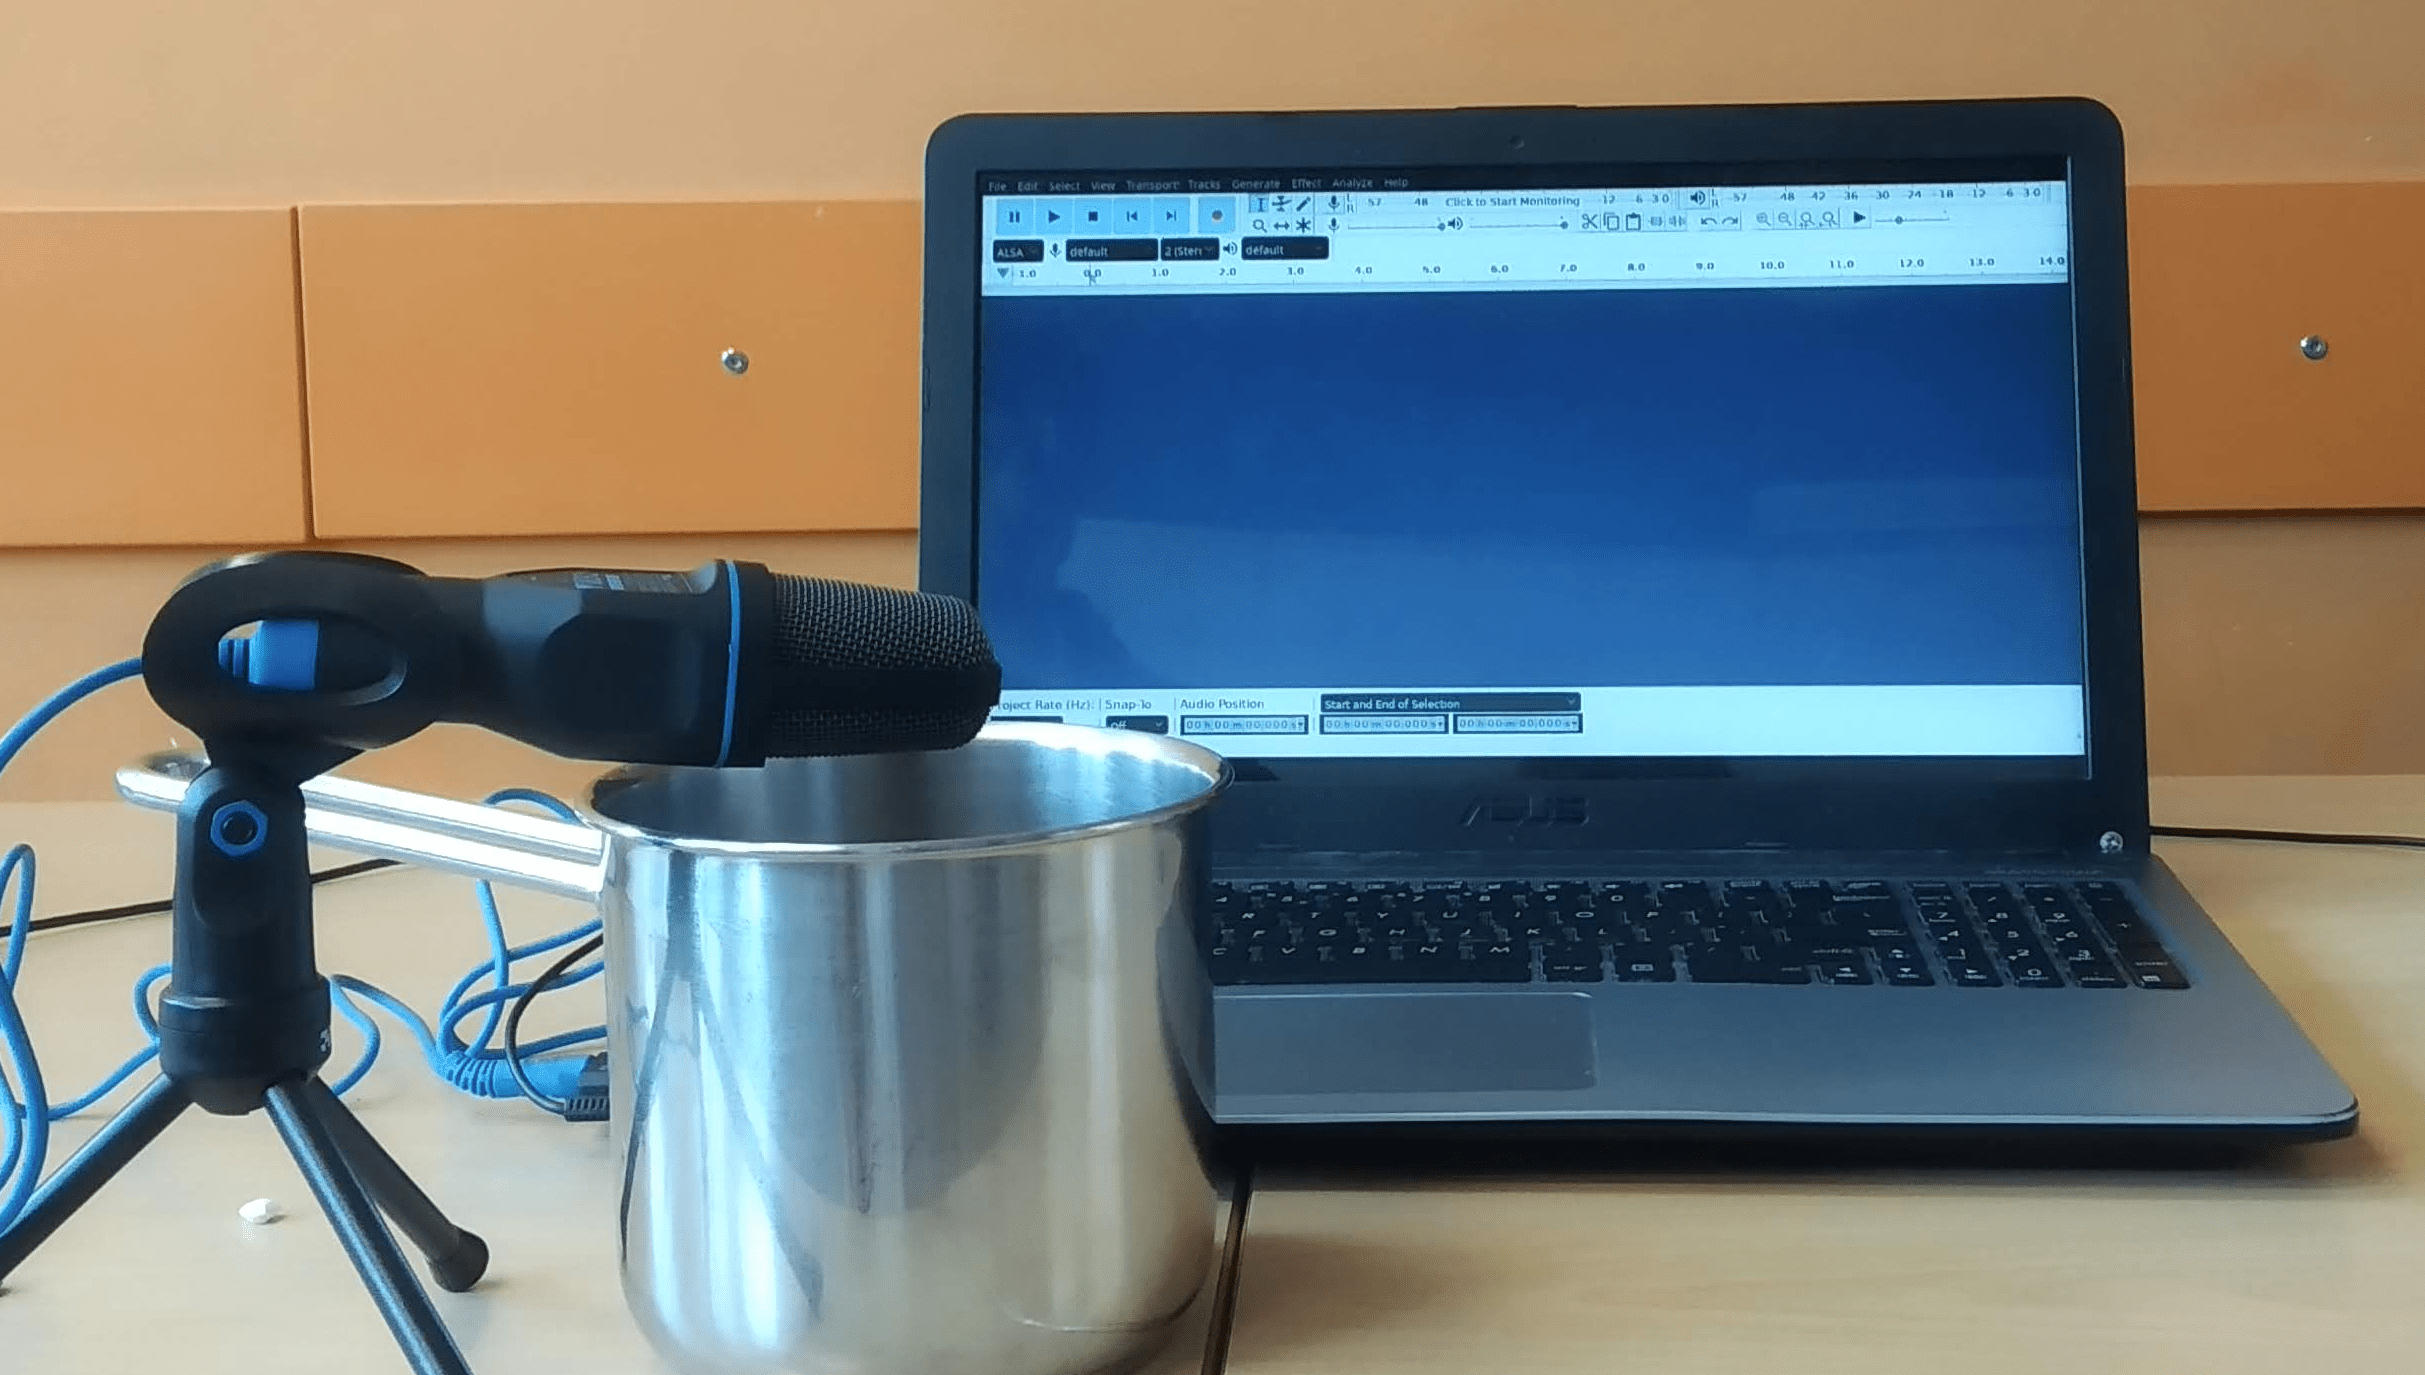
\includegraphics[scale=0.085]{setup.png}
\caption{Setup of the experiment}
\label{setup}
\end{figure}

The setup for the experiment consisted of using a microphone connected to a personal computer to record the sound made by dropping a small rock into the chosen container to excite the natural oscillations (see Fig.\ref{setup}).

The microphone used was a Trust All-round USB Mico microphone. It was tested to be sensitive to frequencies up to about $7000 \, \mathrm{Hz}$.

The audio files were then processed with the audio processing software Audacity [ver. 2.2.1], specifically using its Analyze Spectrum tool to generate the spectrum of the oscillations. The specific settings for the \texttt{Algorithm}, \texttt{Function} and \texttt{Size} fields were \texttt{Spectrum}, \texttt{Hamming window} and \texttt{8192}, respectively.

Measurements were done in two ways. Once by just normally dropping the stone into the container and the second time by trying to block out most of the volume oscillations with a large dampener, like a bottle of water. This way if we plot both spectra we can easily identify which peaks are coming from volume oscillations and which are coming from oscillations of the sides and bottom.

\noindent
The containers used were
%
\begin{enumerate}
\itemsep-0.3em
%
\item Cylindrical cooking pot ($H = 11.0 \, \mathrm{cm}$, $R = 6.0 \, \mathrm{cm}$) [Fig.\ref{pot}]
%
\item Cylindrical tea box ($H = 8.0\, \mathrm{cm}$, $R = 3.0\, \mathrm{cm}$) [Fig.\ref{tea}]
%
\item Rectangular cake pan ($L_x = 16.0 \, \mathrm{cm}$, $L_y =8.0 \, \mathrm{cm}$, $L_z =7.0 \, \mathrm{cm}$) [Fig.\ref{rect}]
%
\item Two mystery containers [Fig.\ref{mys2} and \ref{mys3}]
\end{enumerate} 

\begin{figure}[H]
\centering
\captionsetup{justification=centering}
\captionsetup[subfigure]{justification=centering}
%
\begin{subfigure}{0.25\textwidth}
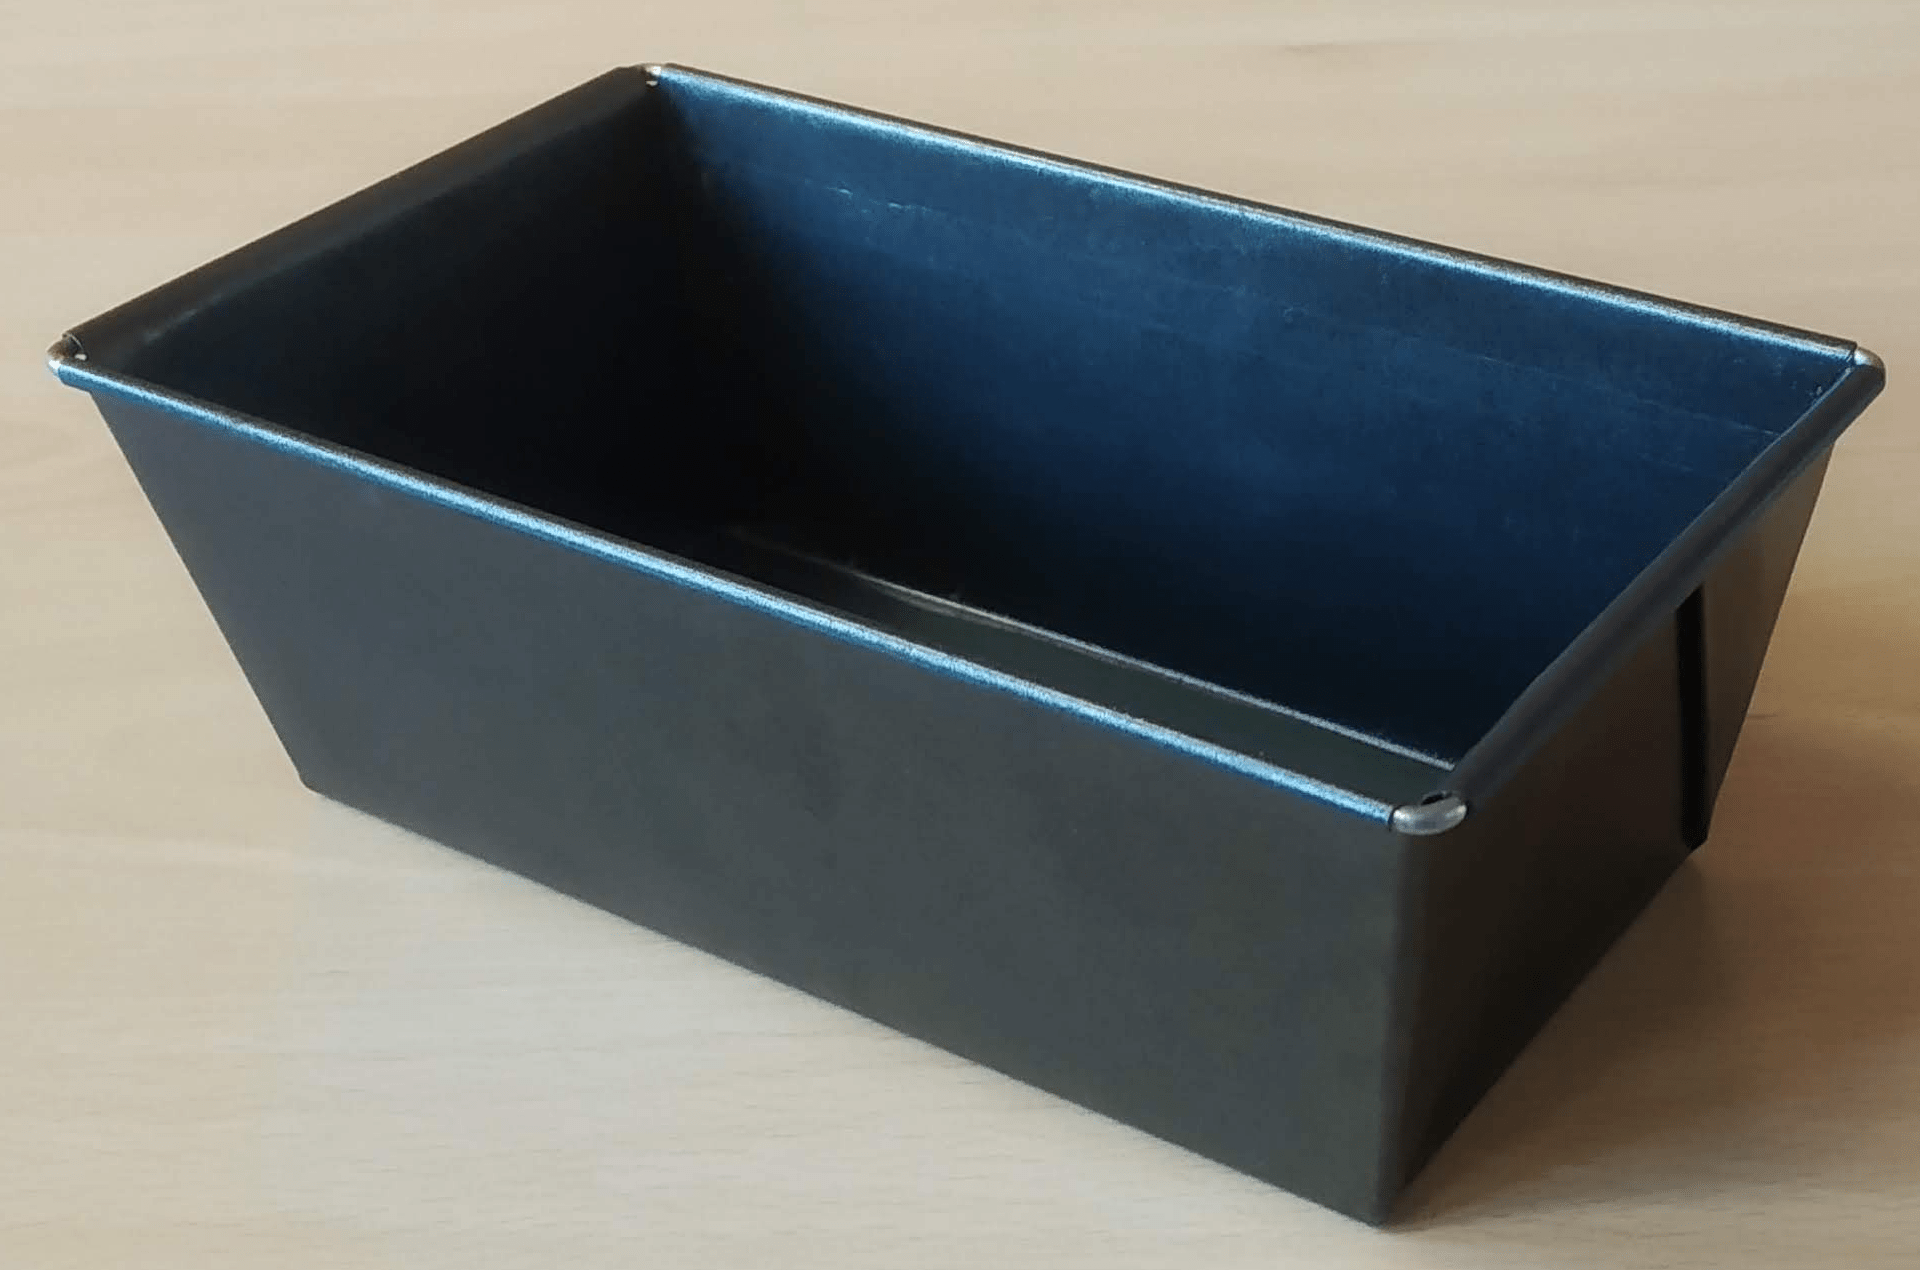
\includegraphics[scale=0.06]{rectangular.png}
\caption{Cake pan}
\label{rect}
\end{subfigure}
\hspace*{\fill}
%
\begin{subfigure}{0.15\textwidth}
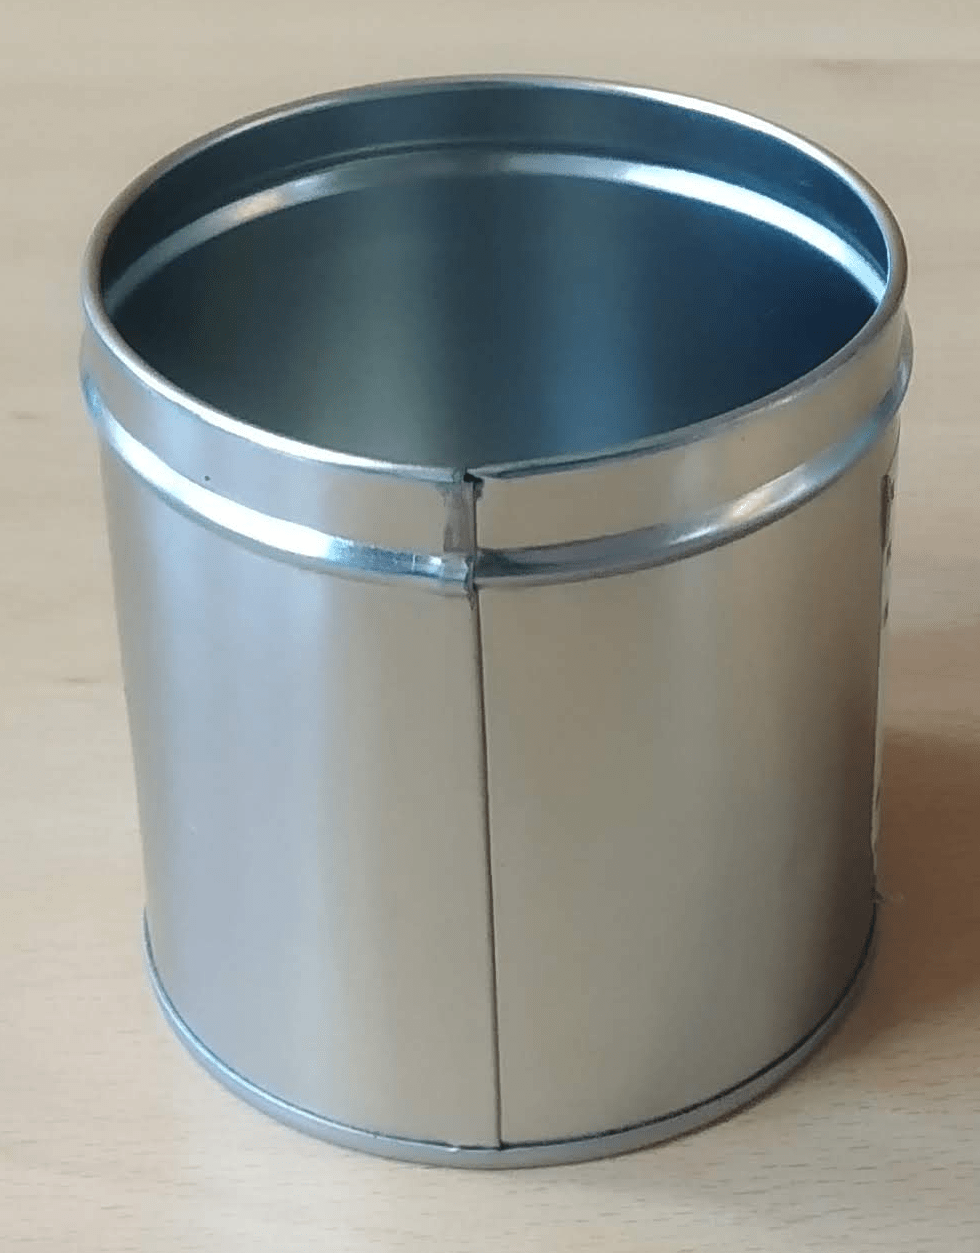
\includegraphics[scale=0.065]{teabox.png}
\caption{Tea box}
\label{tea}
\end{subfigure}
\vskip\baselineskip
%
\begin{subfigure}{0.20\textwidth}
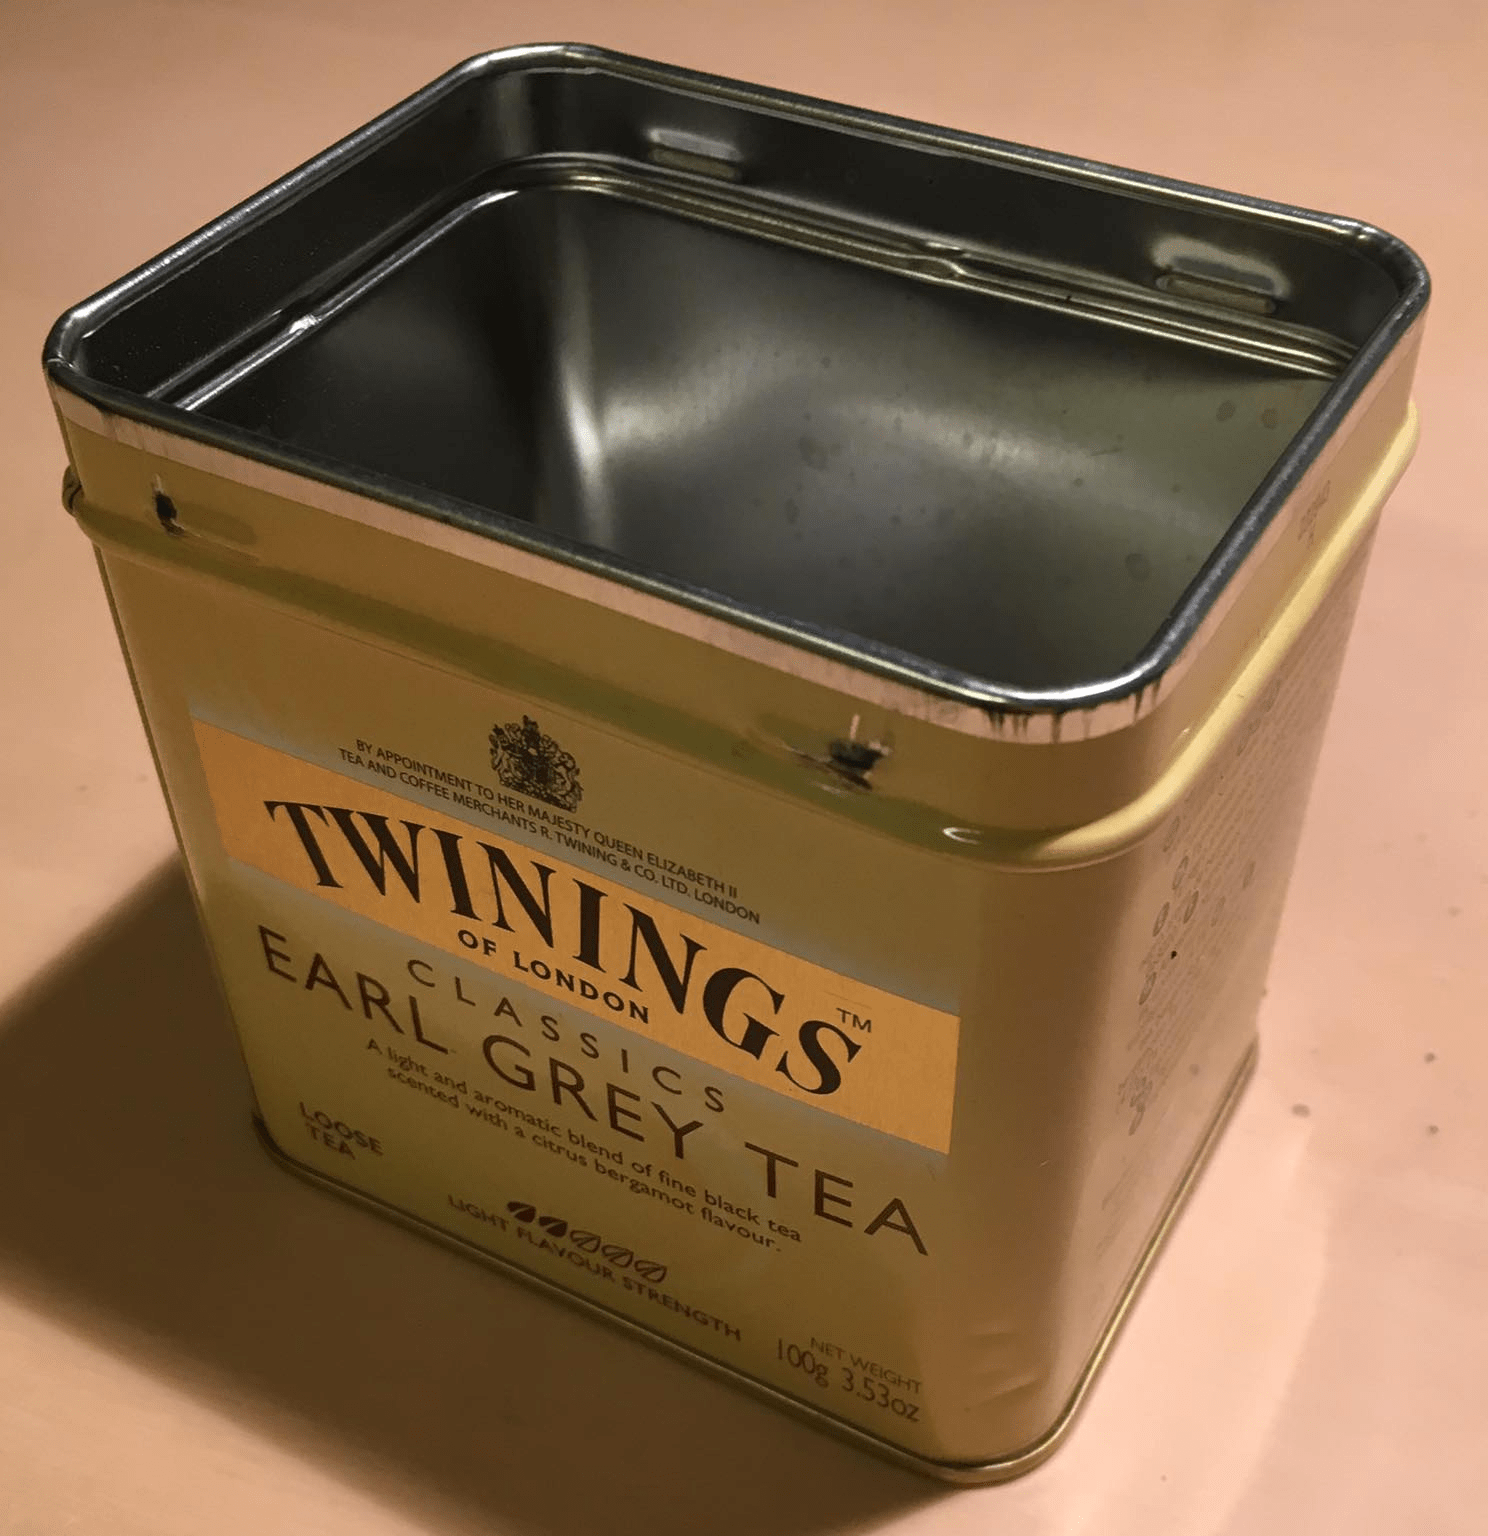
\includegraphics[scale=0.065]{mystery2.png}
\caption{Mystery box 1}
\label{mys2}
\end{subfigure}
\hspace*{\fill}
%
\begin{subfigure}{0.17\textwidth}
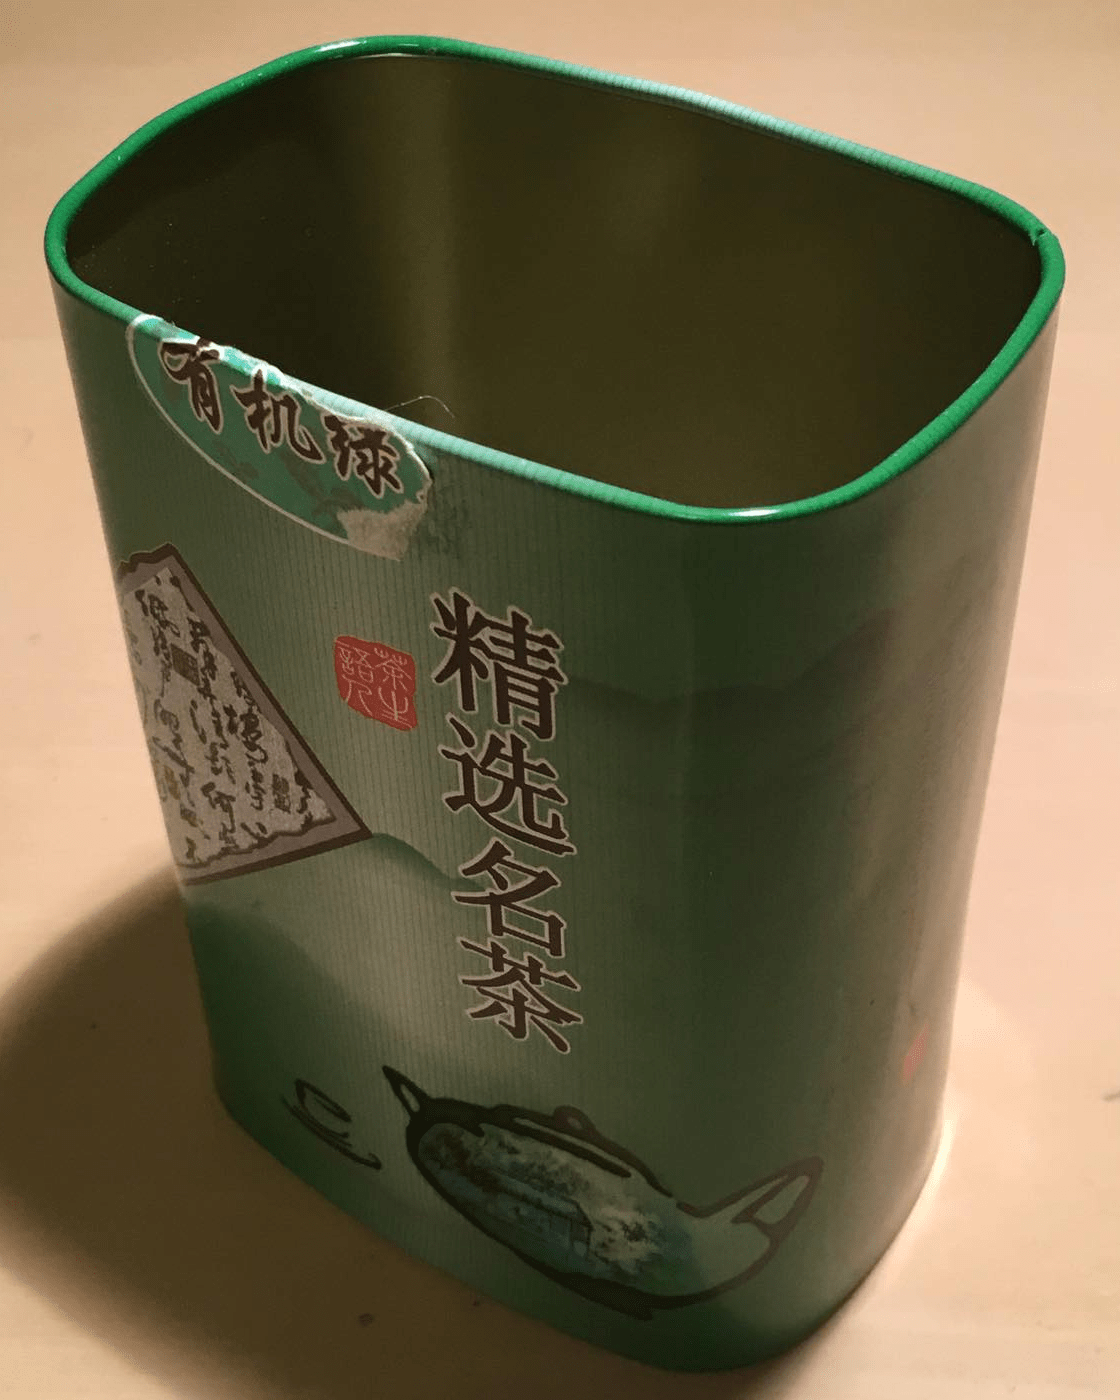
\includegraphics[scale=0.065]{mystery3.png}
\caption{Mystery box 2}
\label{mys3}
\end{subfigure}
%
\begin{subfigure}{0.19\textwidth}
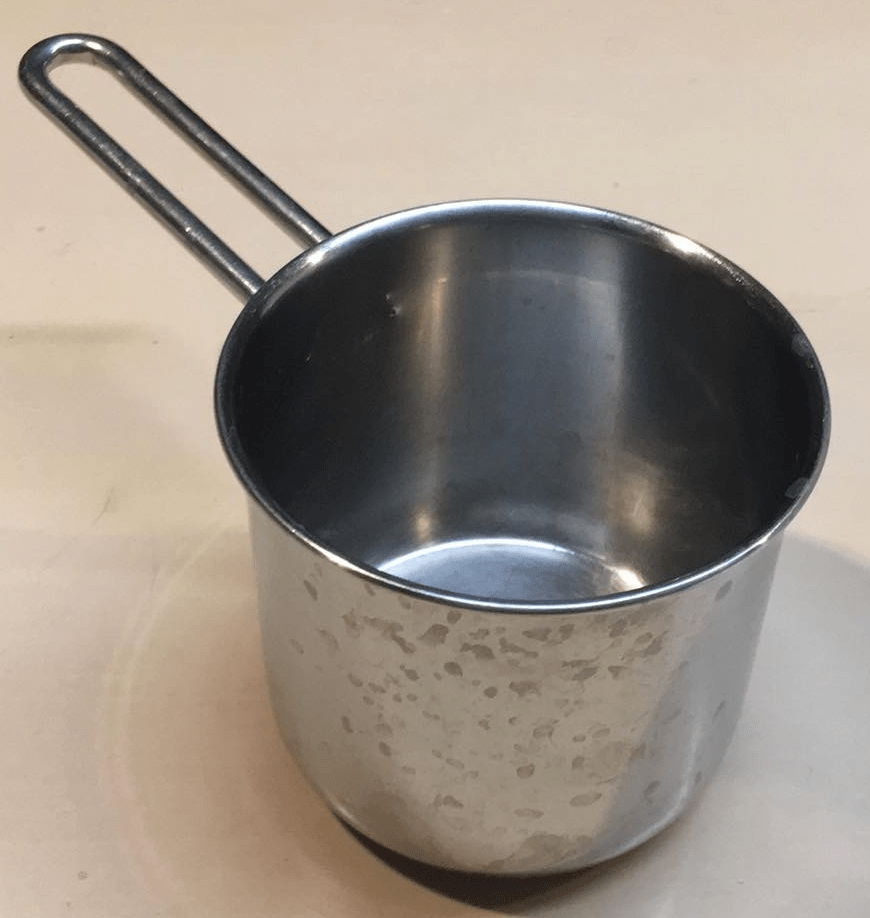
\includegraphics[scale=0.1]{pot.png}
\caption{Cooking pot}
\label{pot}
\end{subfigure}
%
\caption{Containers used in the experiment}
\label{containers}
\end{figure}

The last two mystery boxes were a mystery in the sense that the only information made available to the experimenter were audio files of sounds from the containers being hit. From this they tried to determine the geometrical properties and dimensions. This served as a way of removing the bias of the experimenter when trying to fit resonance peaks onto an actual experimental spectrum.

\section{Experimental results}

One of the five containers, namely the cooking pot, was used to test whether the ideas presented above worked in practice. We did this by measuring its dimensions and trying to fit the measured spectrum with the theory. The precise dimensions of the pot were $H = (11.0 \pm 0.1) \, \mathrm{cm}$ and $R = (6.0 \pm 0.1) \, \mathrm{cm}$ which makes the effective height of the pot $H' = (14.6 \pm 0.2) \, \mathrm{cm}$. In this spectrum, as in the others, the speed of sound was taken to be $c = (343 \pm 2) \, \mathrm{m/s}$. The theoretical predictions with their respective errors and the positions of the most prominent peaks from both the blocked and normal spectra are plotted in Fig.\ref{potpeaks}.

\begin{figure}[H]
\centering
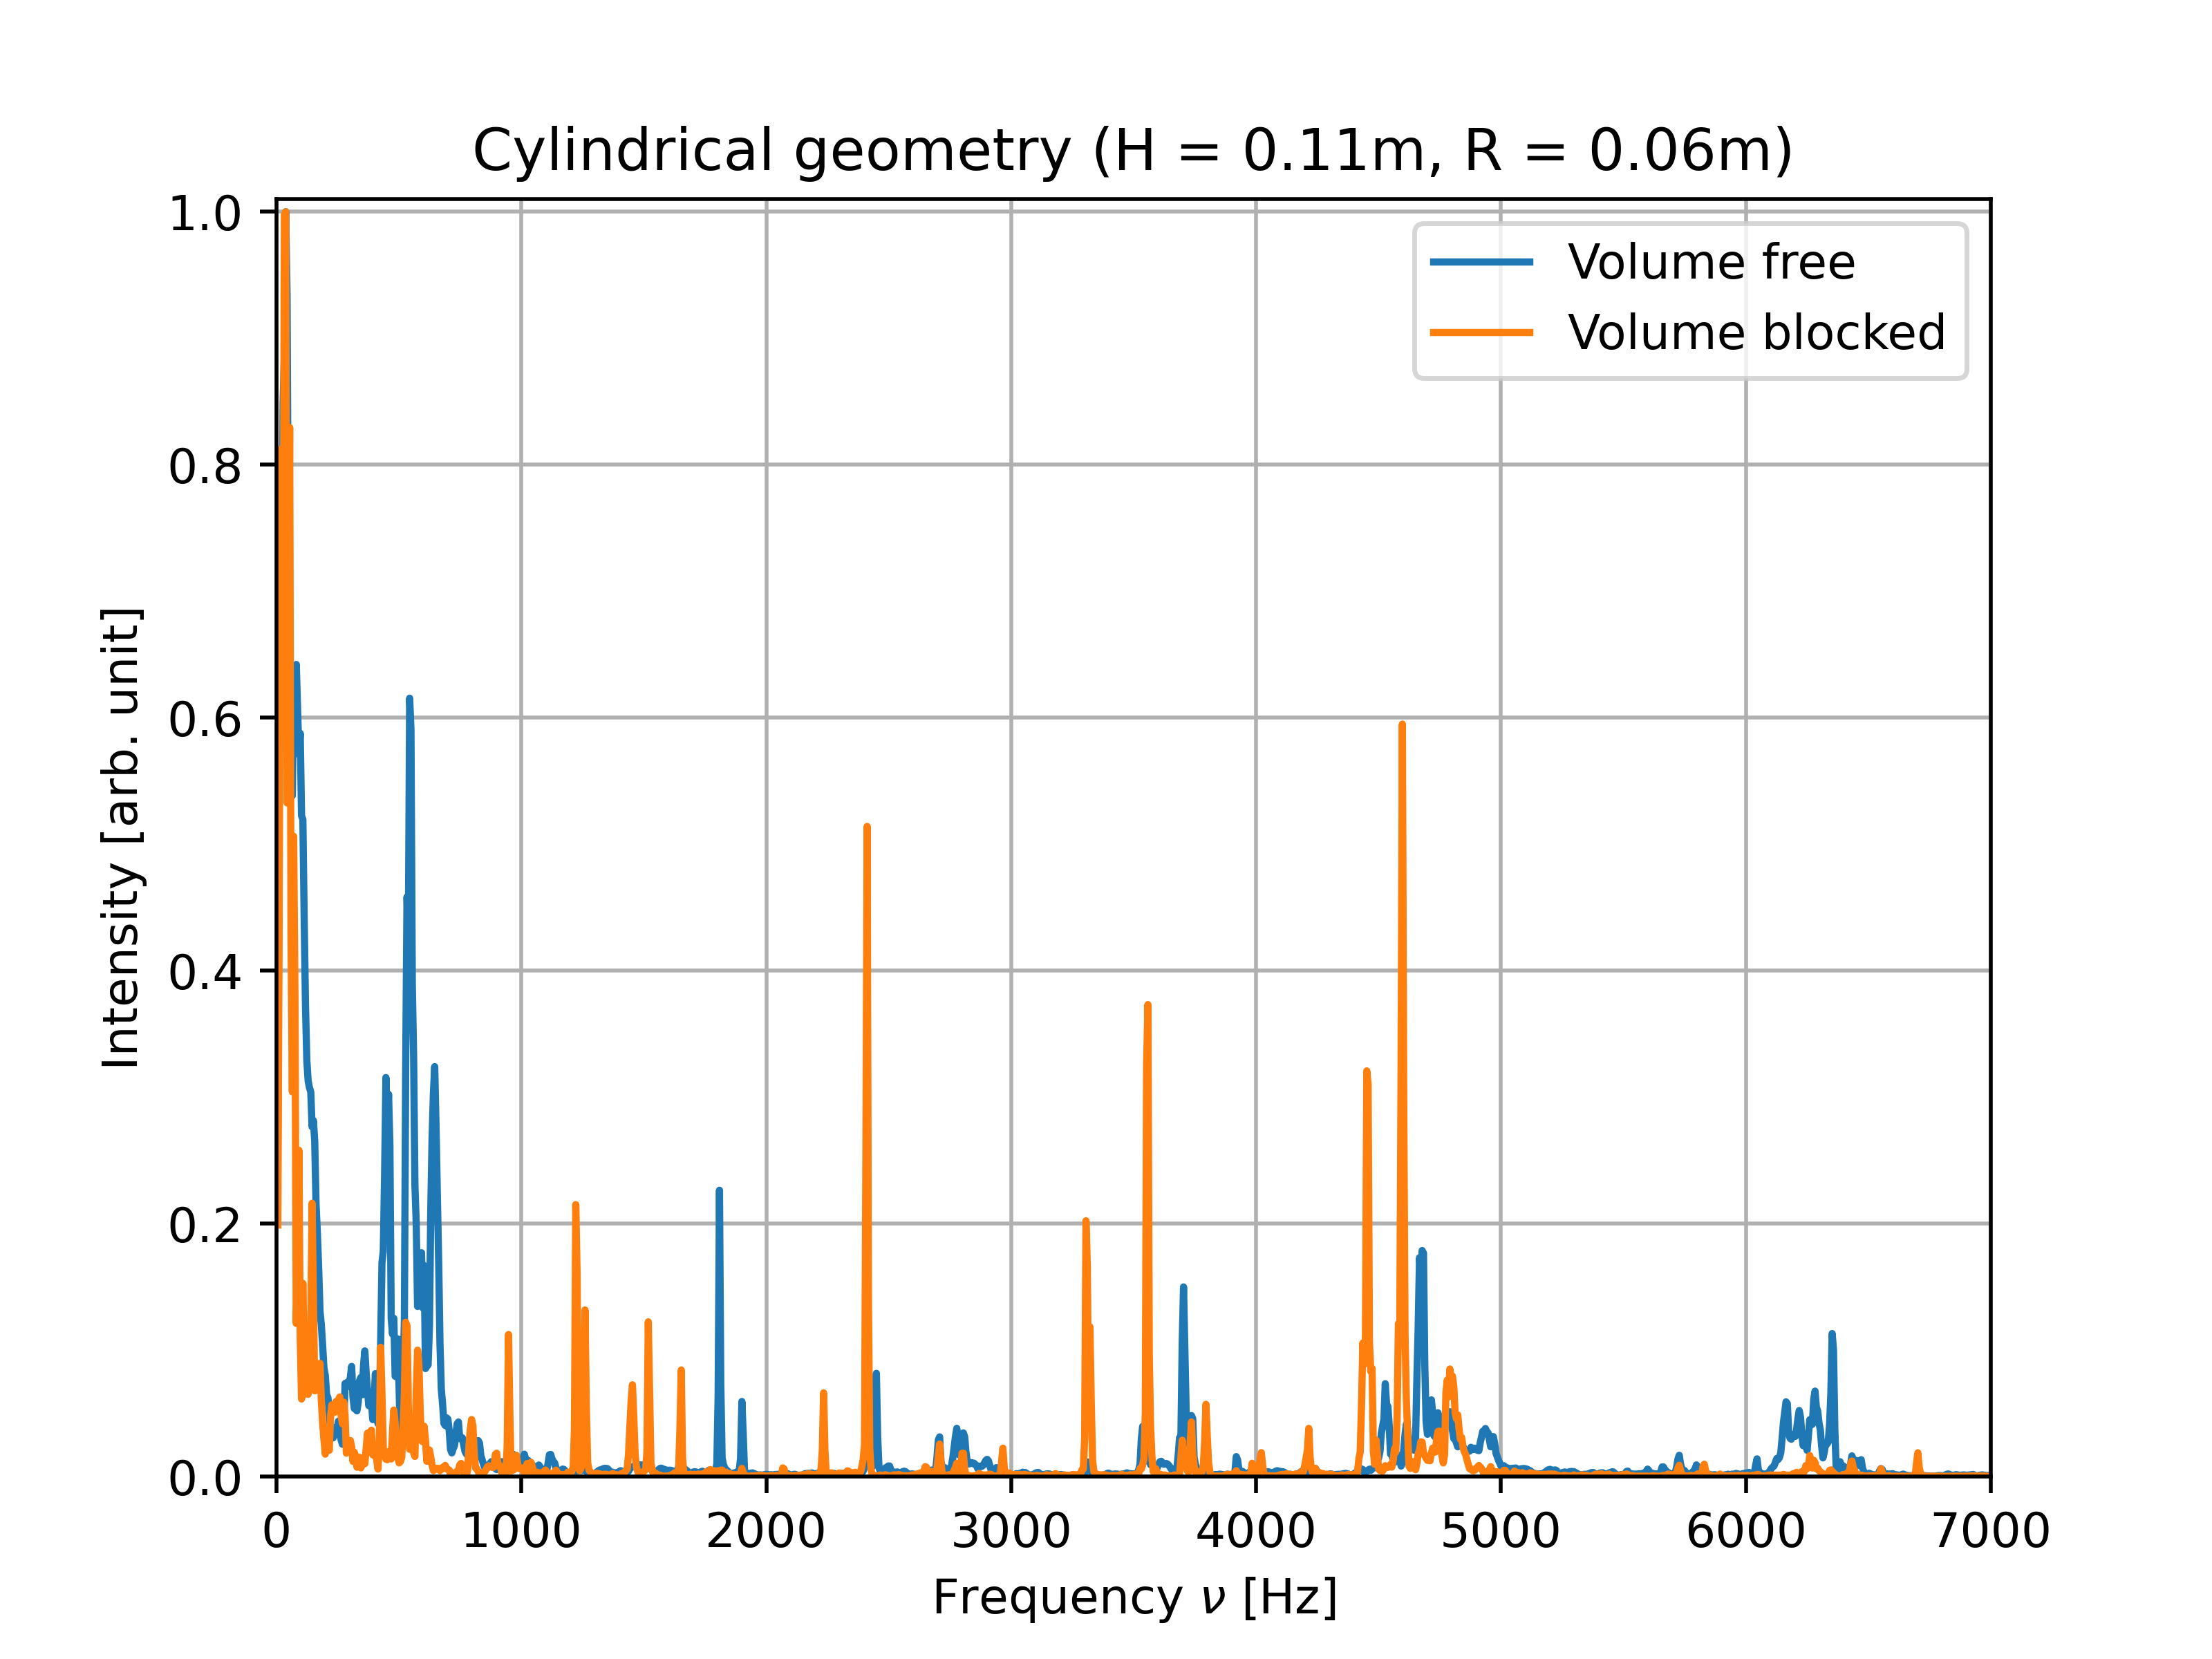
\includegraphics[scale=0.0305]{potpeaks.png}
\caption{Plot of the theoretical predictions with their associated errors coming from the geometrical measurements (red) and the most prominent peaks of the blocked (yellow) and free (blue) spectra. Vertical axis has no physical meaning.}
\label{potpeaks}
\end{figure}

The first thing we notice is that for frequencies higher than around $5000 \, \mathrm{Hz}$ the geometrical measurement errors become to large to effectively fit the theory and experiment. At frequencies lower than about $900 \, \mathrm{Hz}$ we have the problem of the spectrum being to noisy. Between these two extremes we are looking for places where the red and blue lines agree. The places where the blue and yellow lines agree can be taken out of the discussion as they are not volume oscillations.

We see that there is some agreement between the two with the notable exceptions of the lines at around $2200 \, \mathrm{Hz}$ and $4100 \, \mathrm{Hz}$. One possible explanation is that these modes just weren't excited with enough energy to show up on the spectrum.  

\begin{figure}
\centering
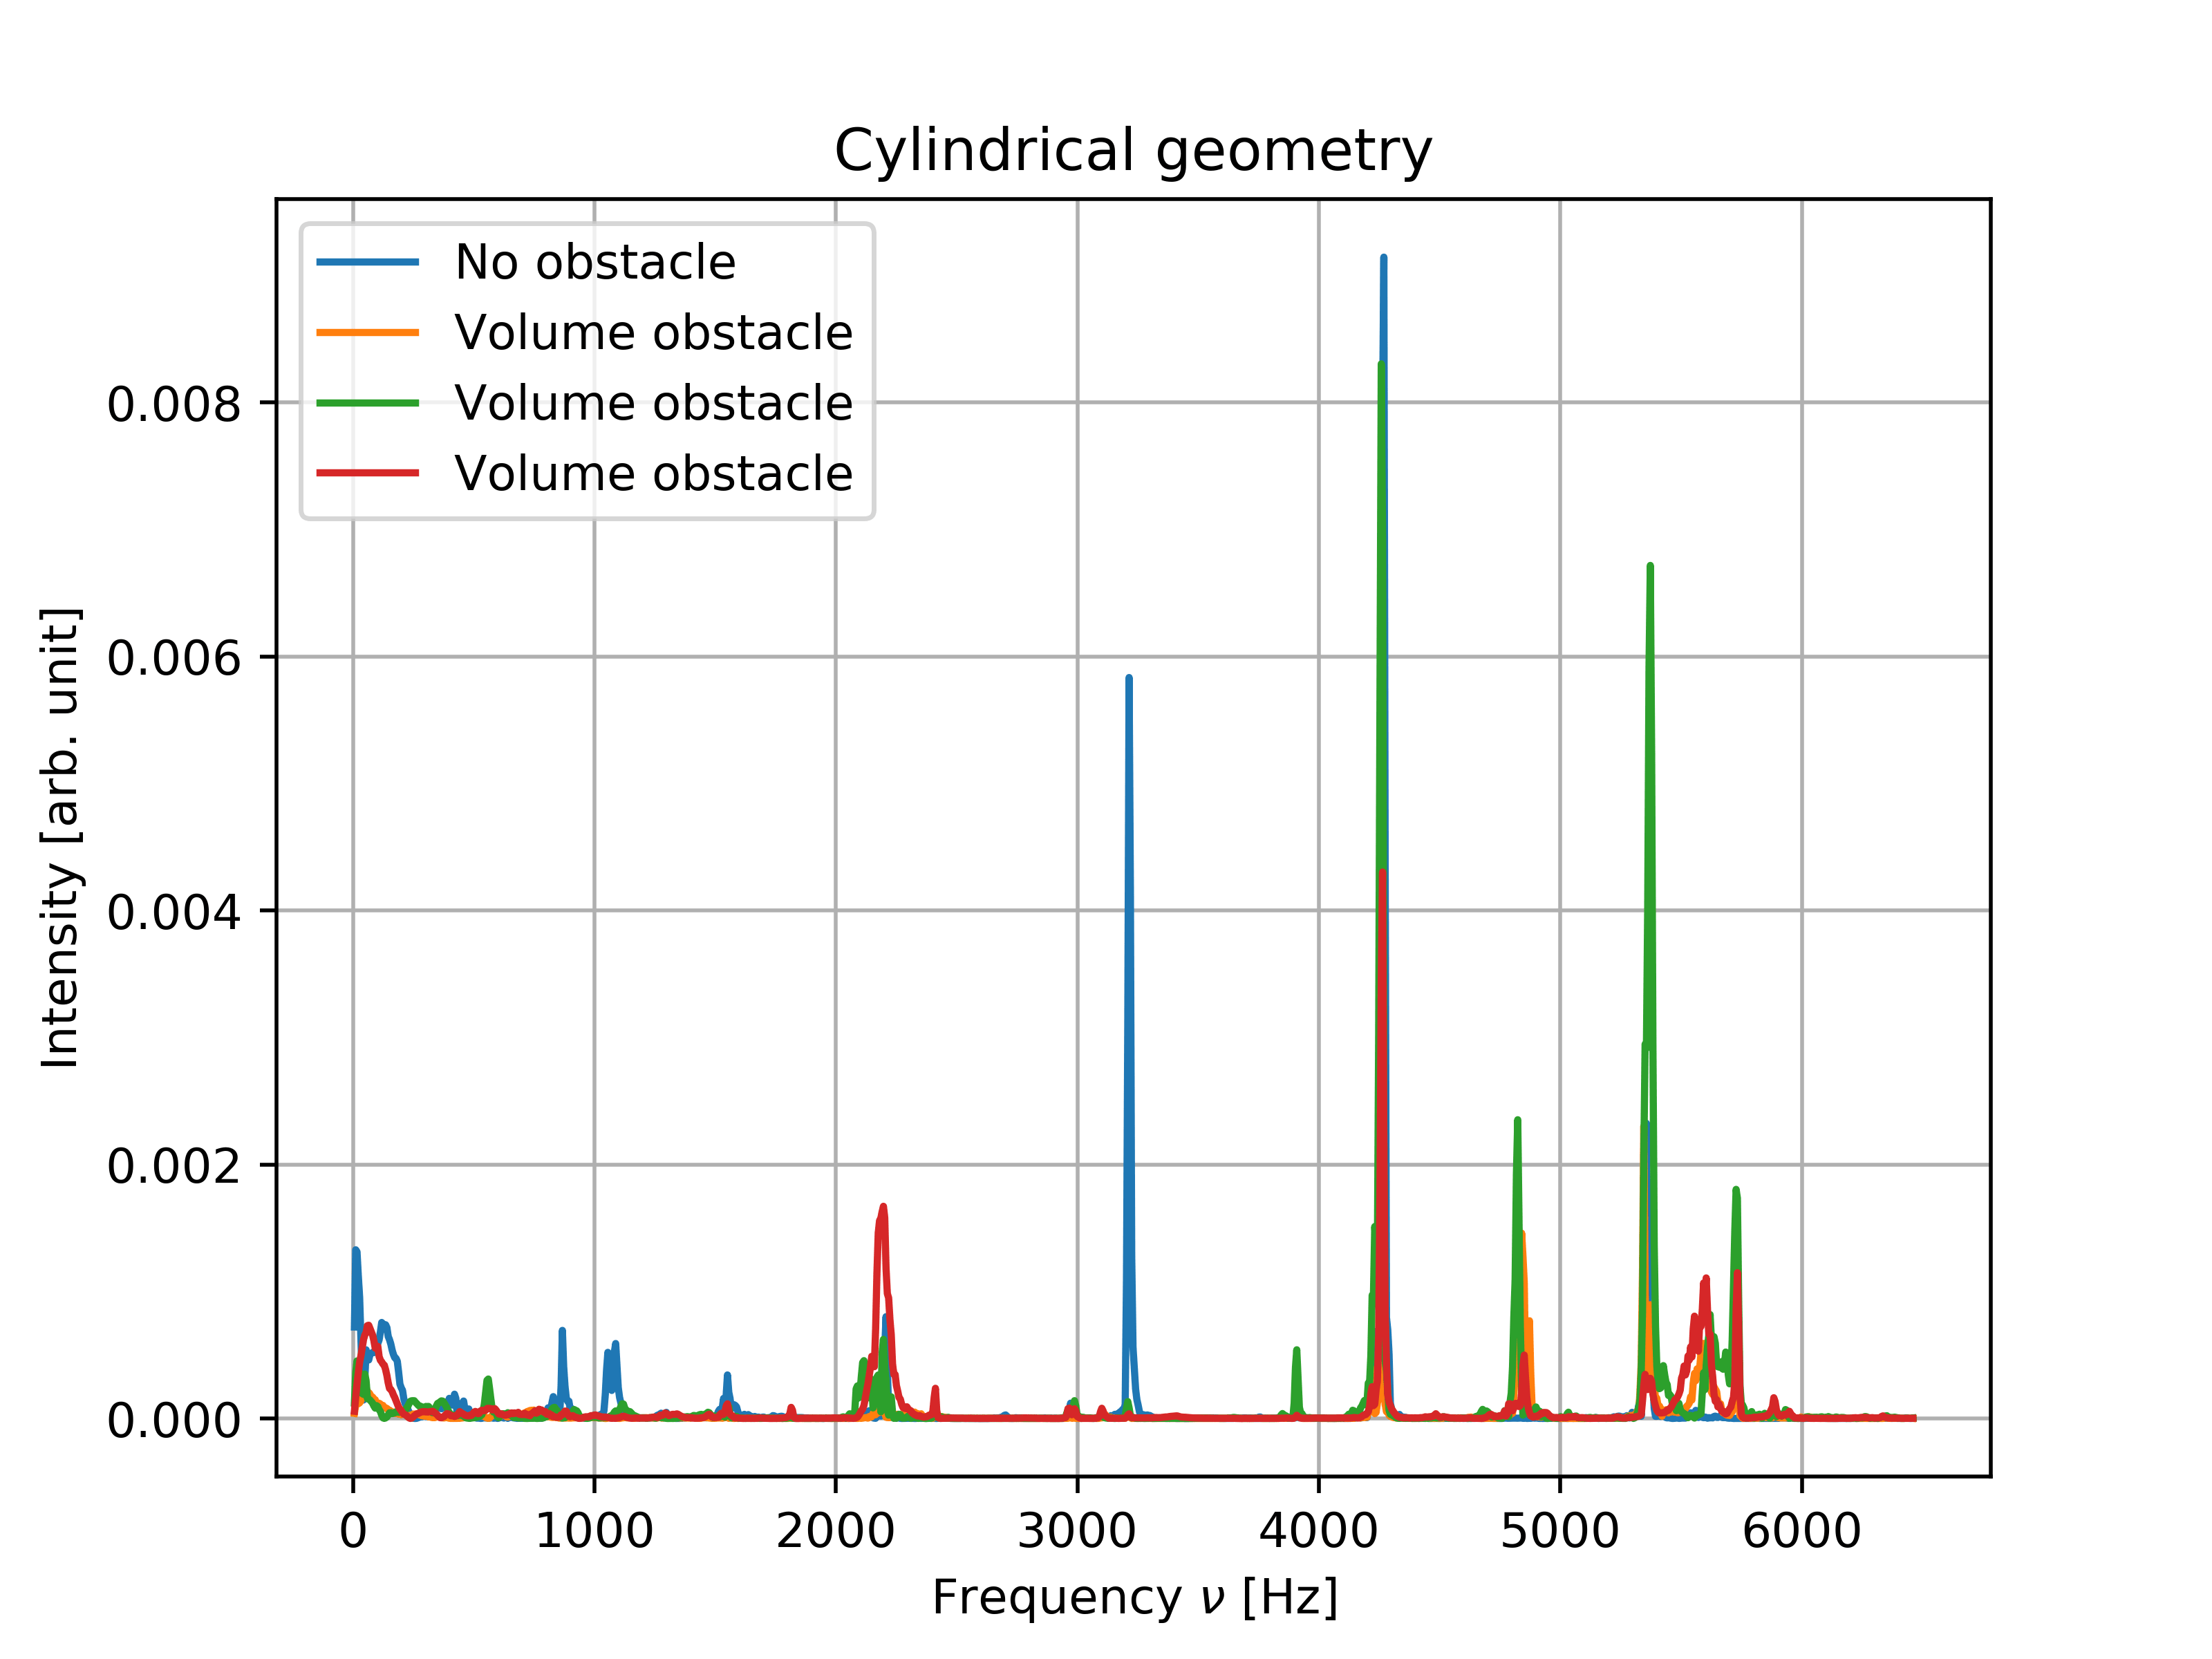
\includegraphics[scale=0.07]{teapeaks.png}
\caption{Plot of the spectrum of the tea box without a blockage (blue) and three measurements with one (orange, green, red). Vertical axis has arbitrary units}
\label{teapeaks}
\end{figure}

From analyzing the tea box spectrum (see Fig.\ref{teapeaks}), we notice peaks at $1055 \, \mathrm{Hz}$ and, to good precision, at three times that frequency $3216 \, \mathrm{Hz}$. This is a dead giveaway for the size of the linear direction of oscillation, giving the value $H' = (8.1 \pm 0.1) \, \mathrm{cm}$. There aren't enough other identifiable peaks to get the radius $R$. Our precision is thus limited because we can't subtract off the end correction, but $H'$ still gives a good guess to the actual height $H$.

\begin{figure}[H]
\centering
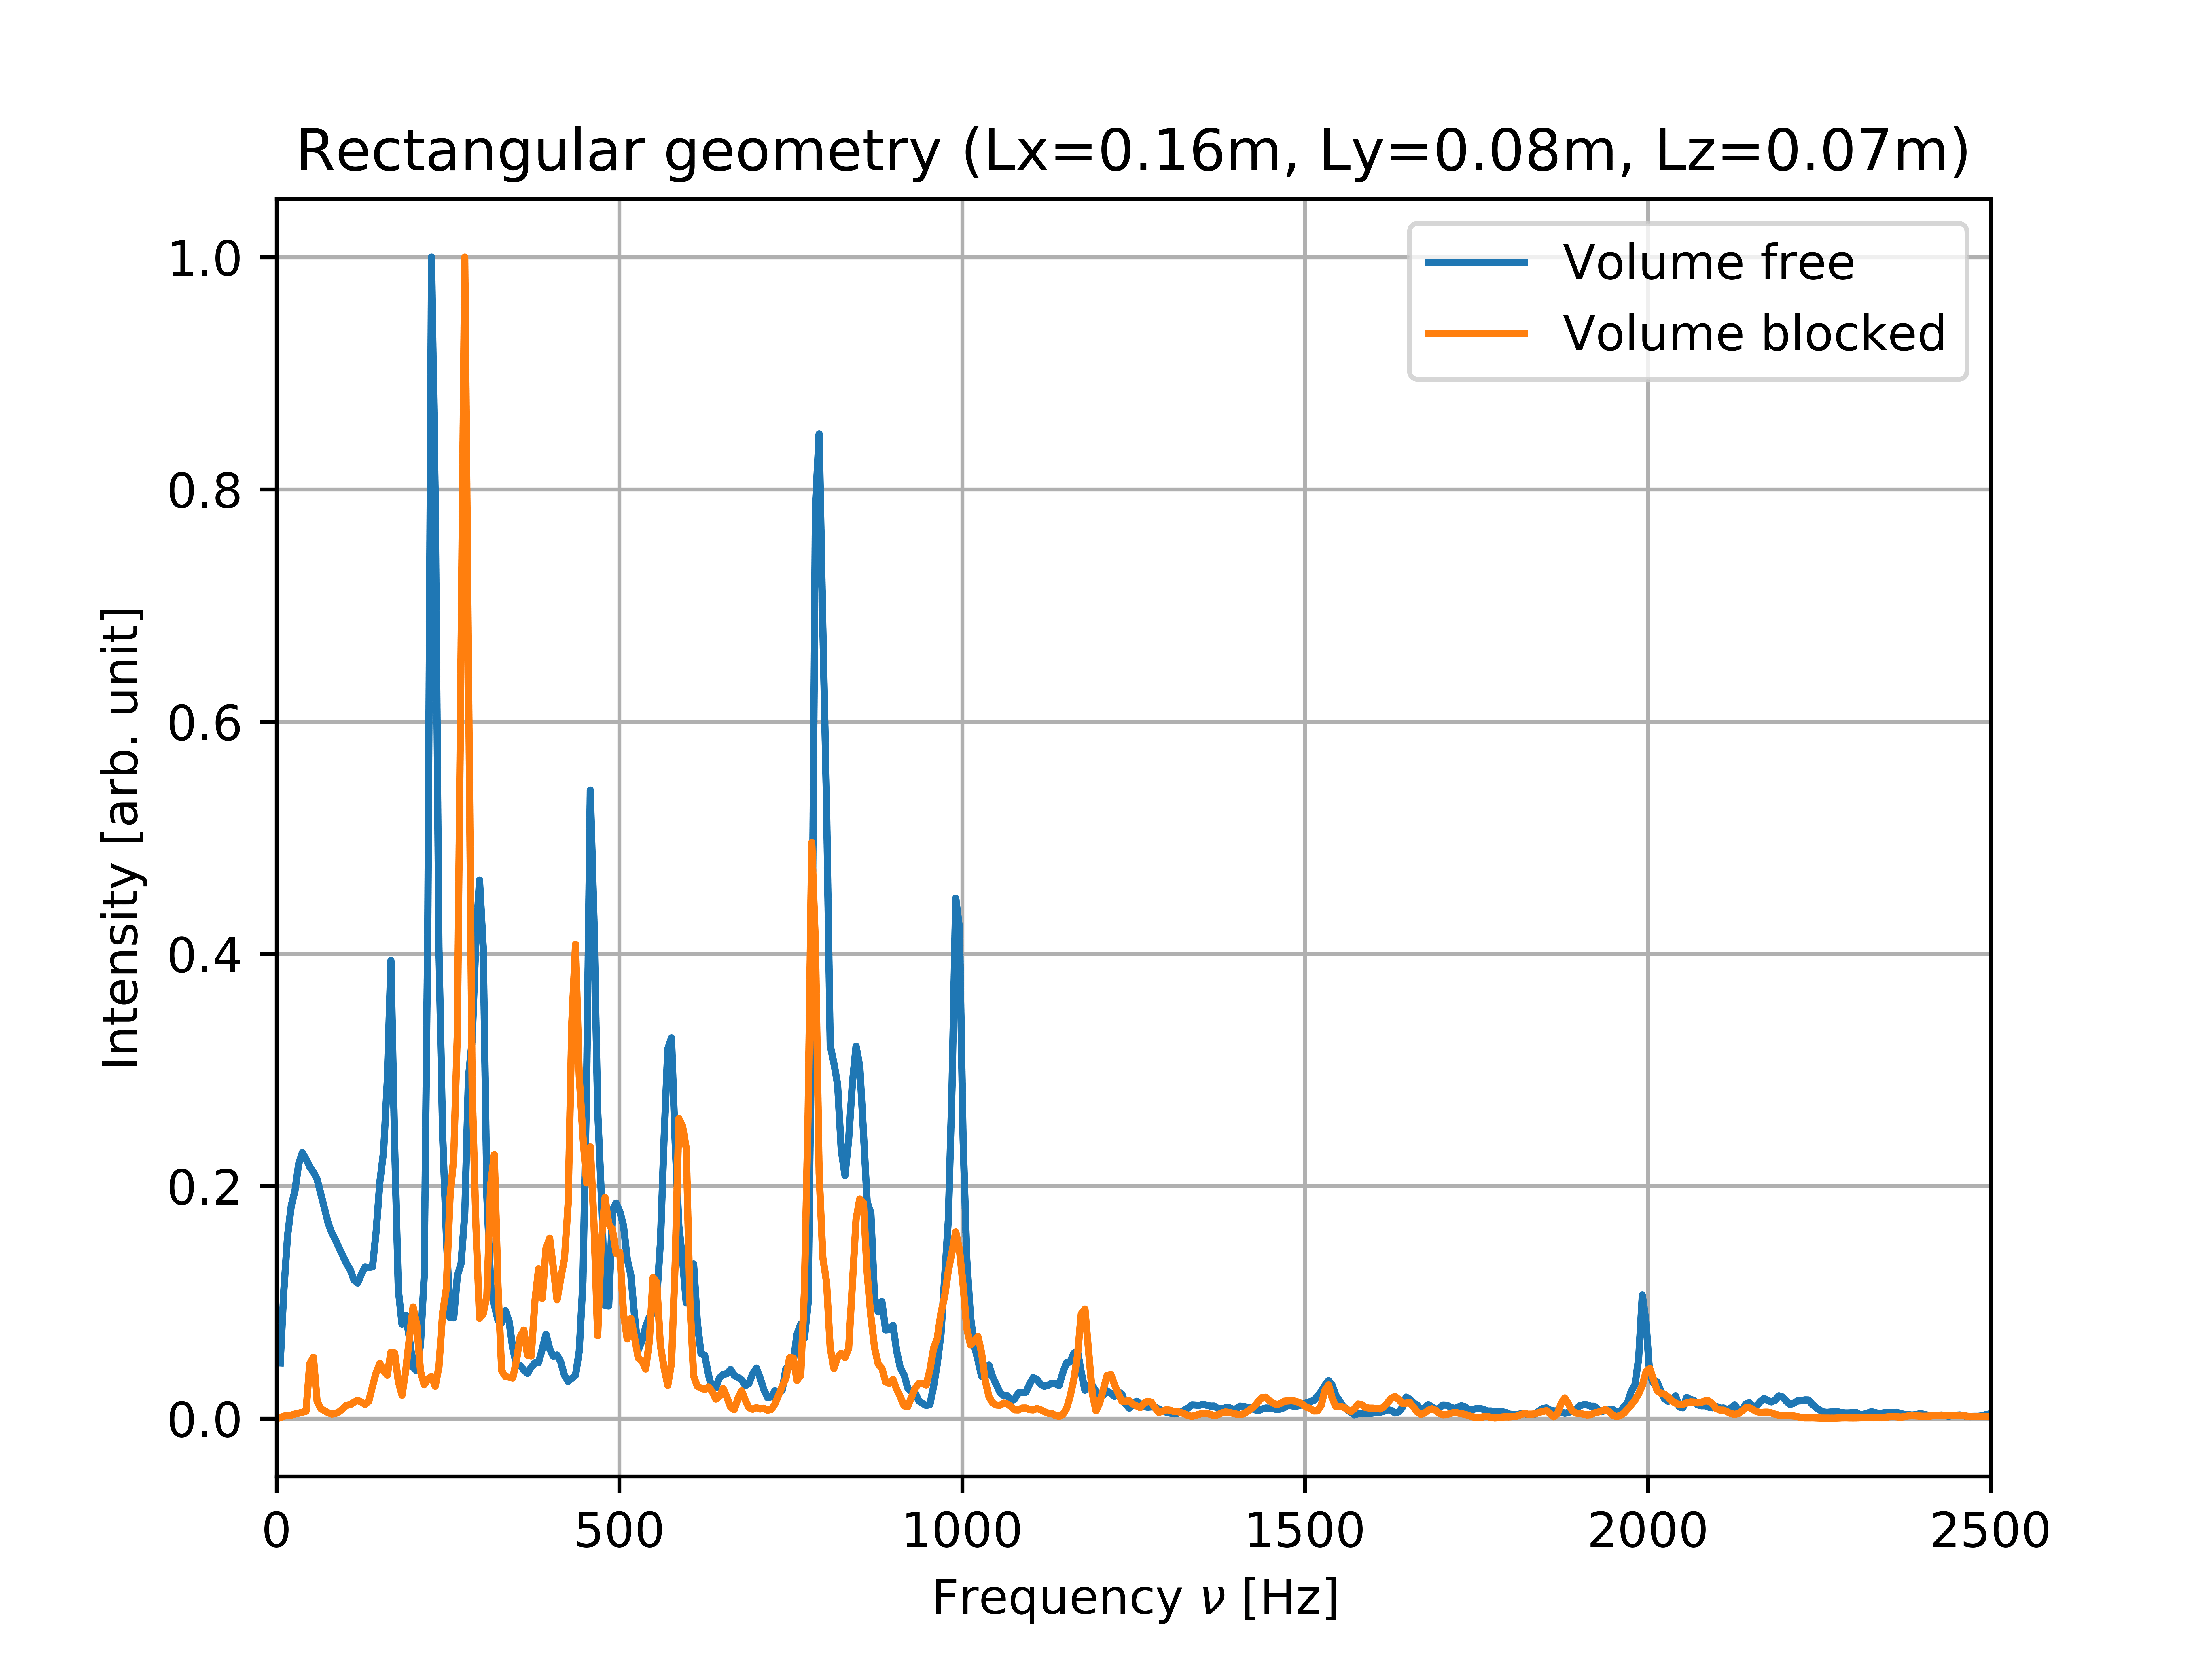
\includegraphics[scale=0.0305]{rectpeaks.png}
\caption{Plot of the spectrum of the rectangular cake pan.}
\label{rectpeaks}
\end{figure}

In the case of the rectangular cake pan (see Fig.\ref{rectpeaks}), we get no recognizable peaks in the spectrum because of all the little ways in which our setup departs from the model. Namely, these are the geometry not being perfectly rectangular, the edges not being perfectly motionless, and the opening giving rise to a condition that isn't Neumann to any degree of accuracy.

\begin{figure}
\centering
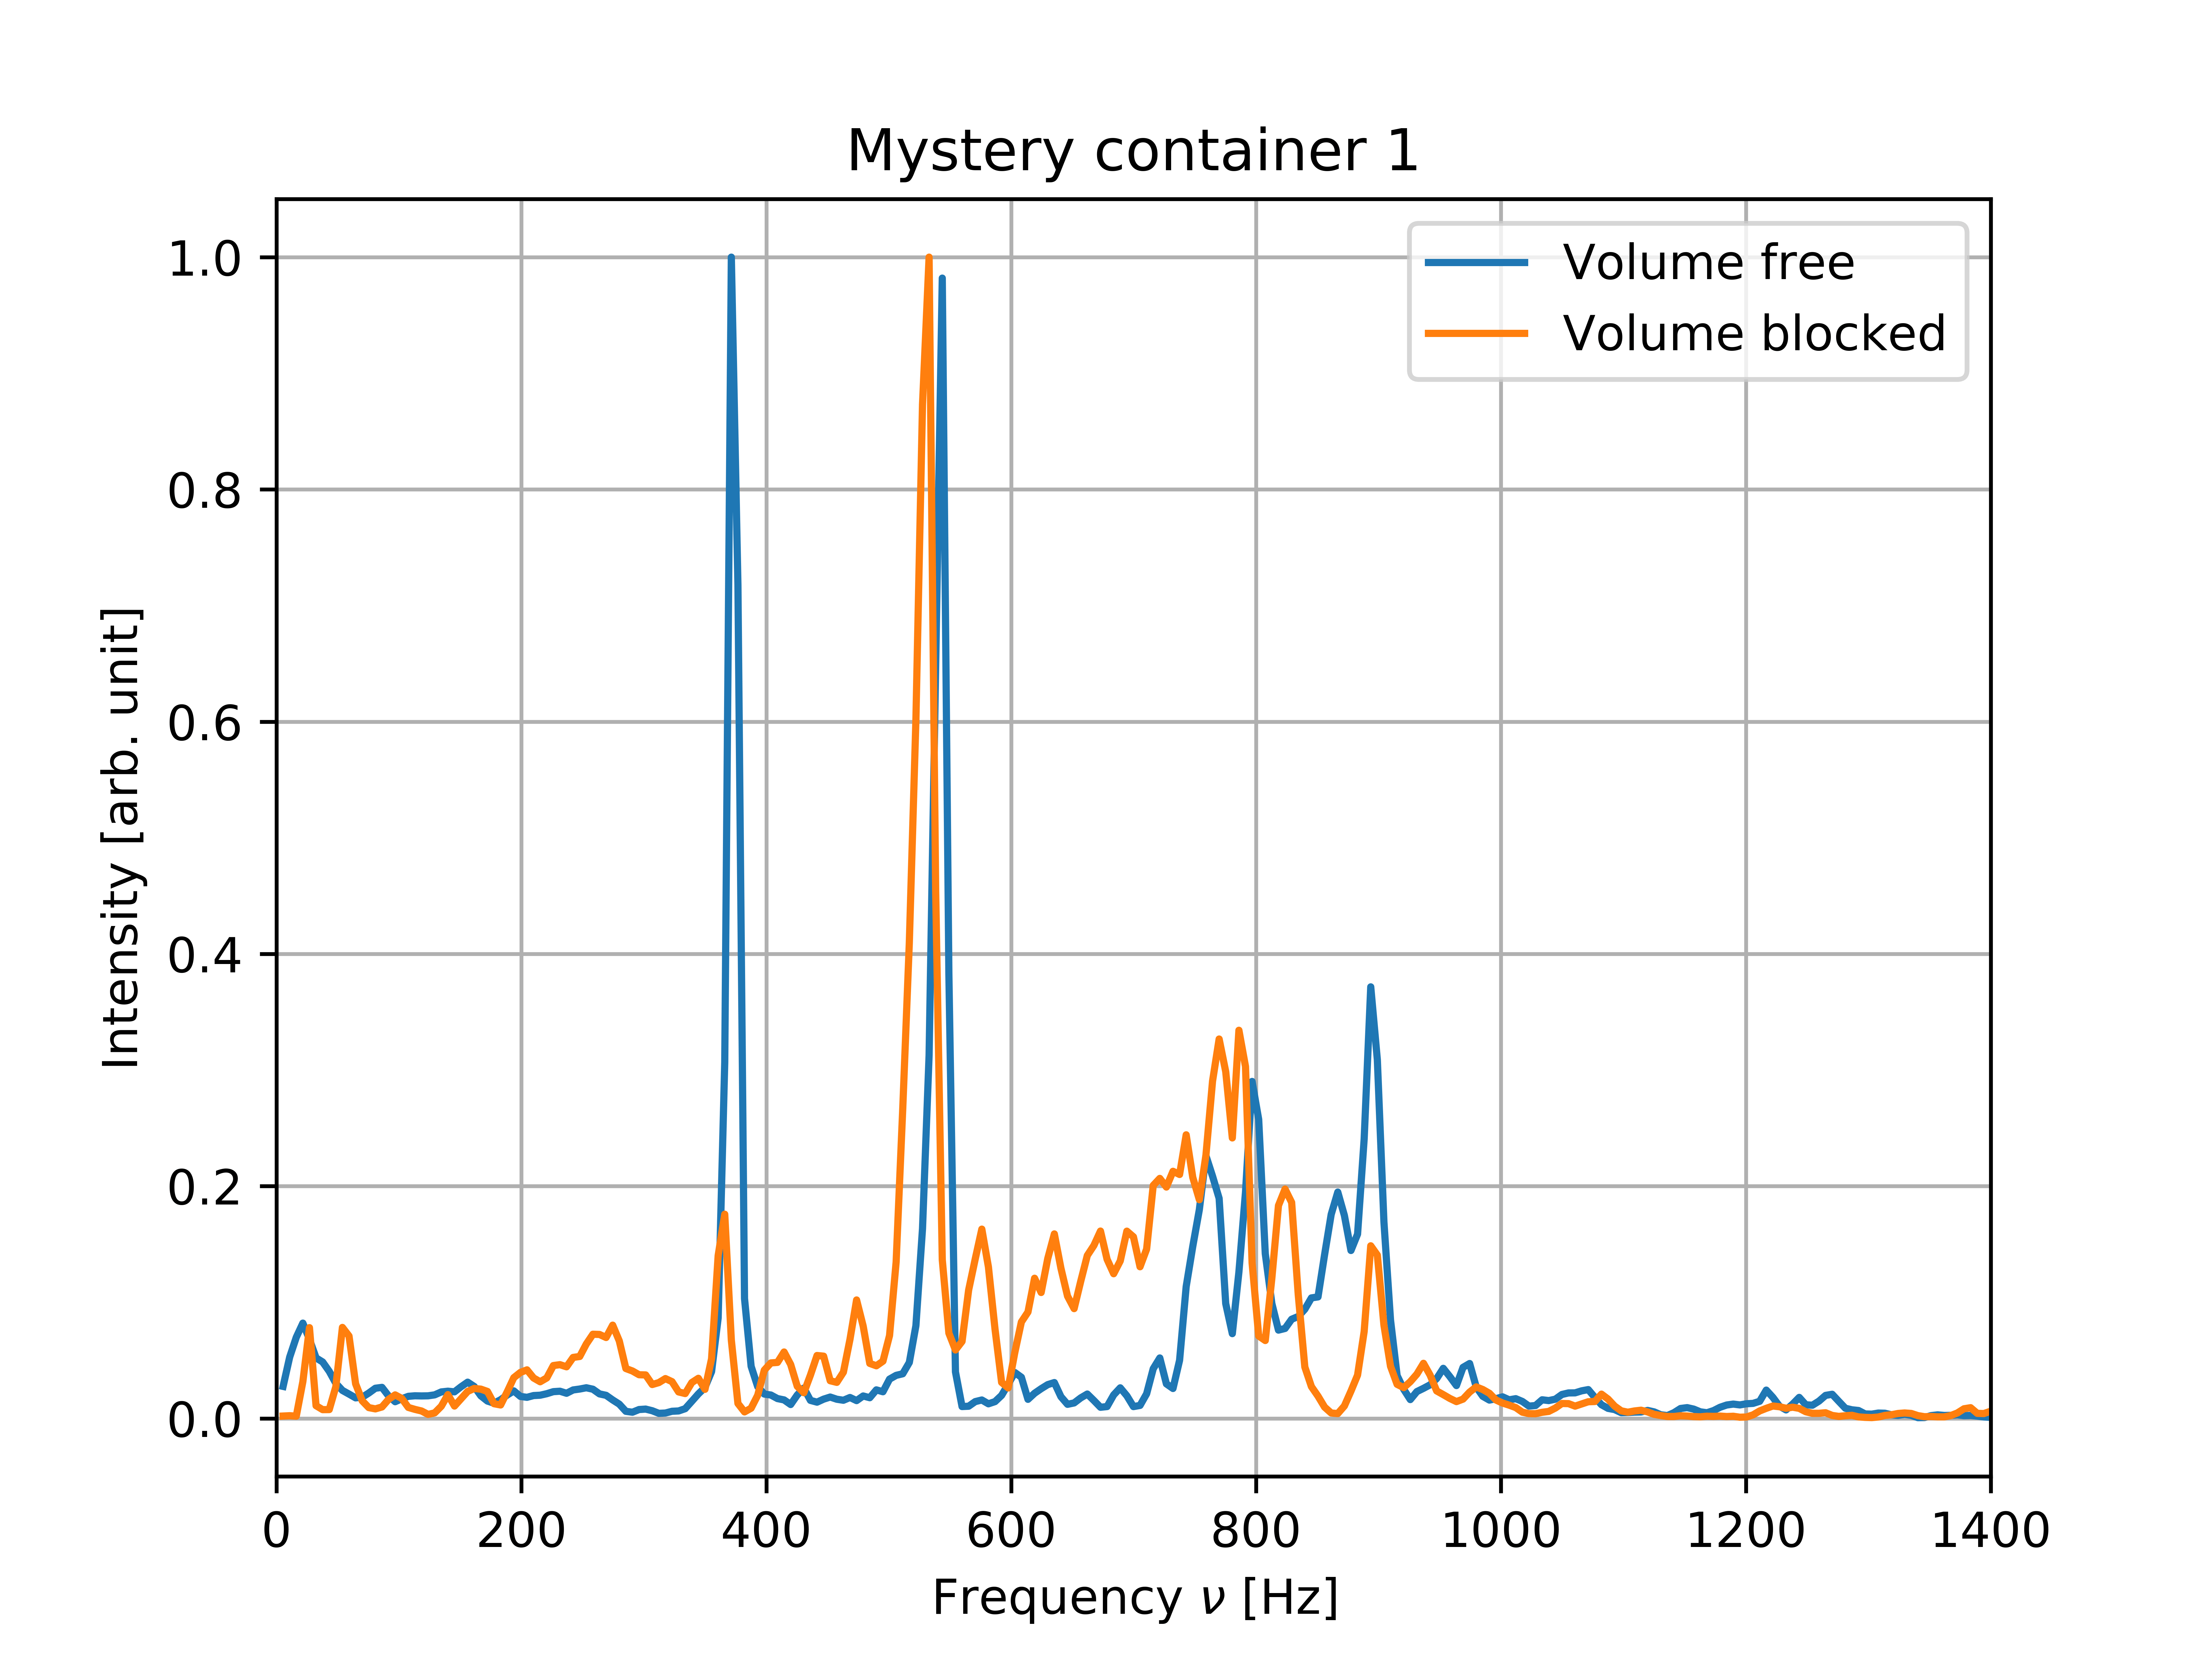
\includegraphics[scale=0.0305]{mystery2peaks.png}
\caption{Plot of the spectrum of mystery box 1.}
\label{mys2peaks}
\end{figure}

\begin{figure}
\centering
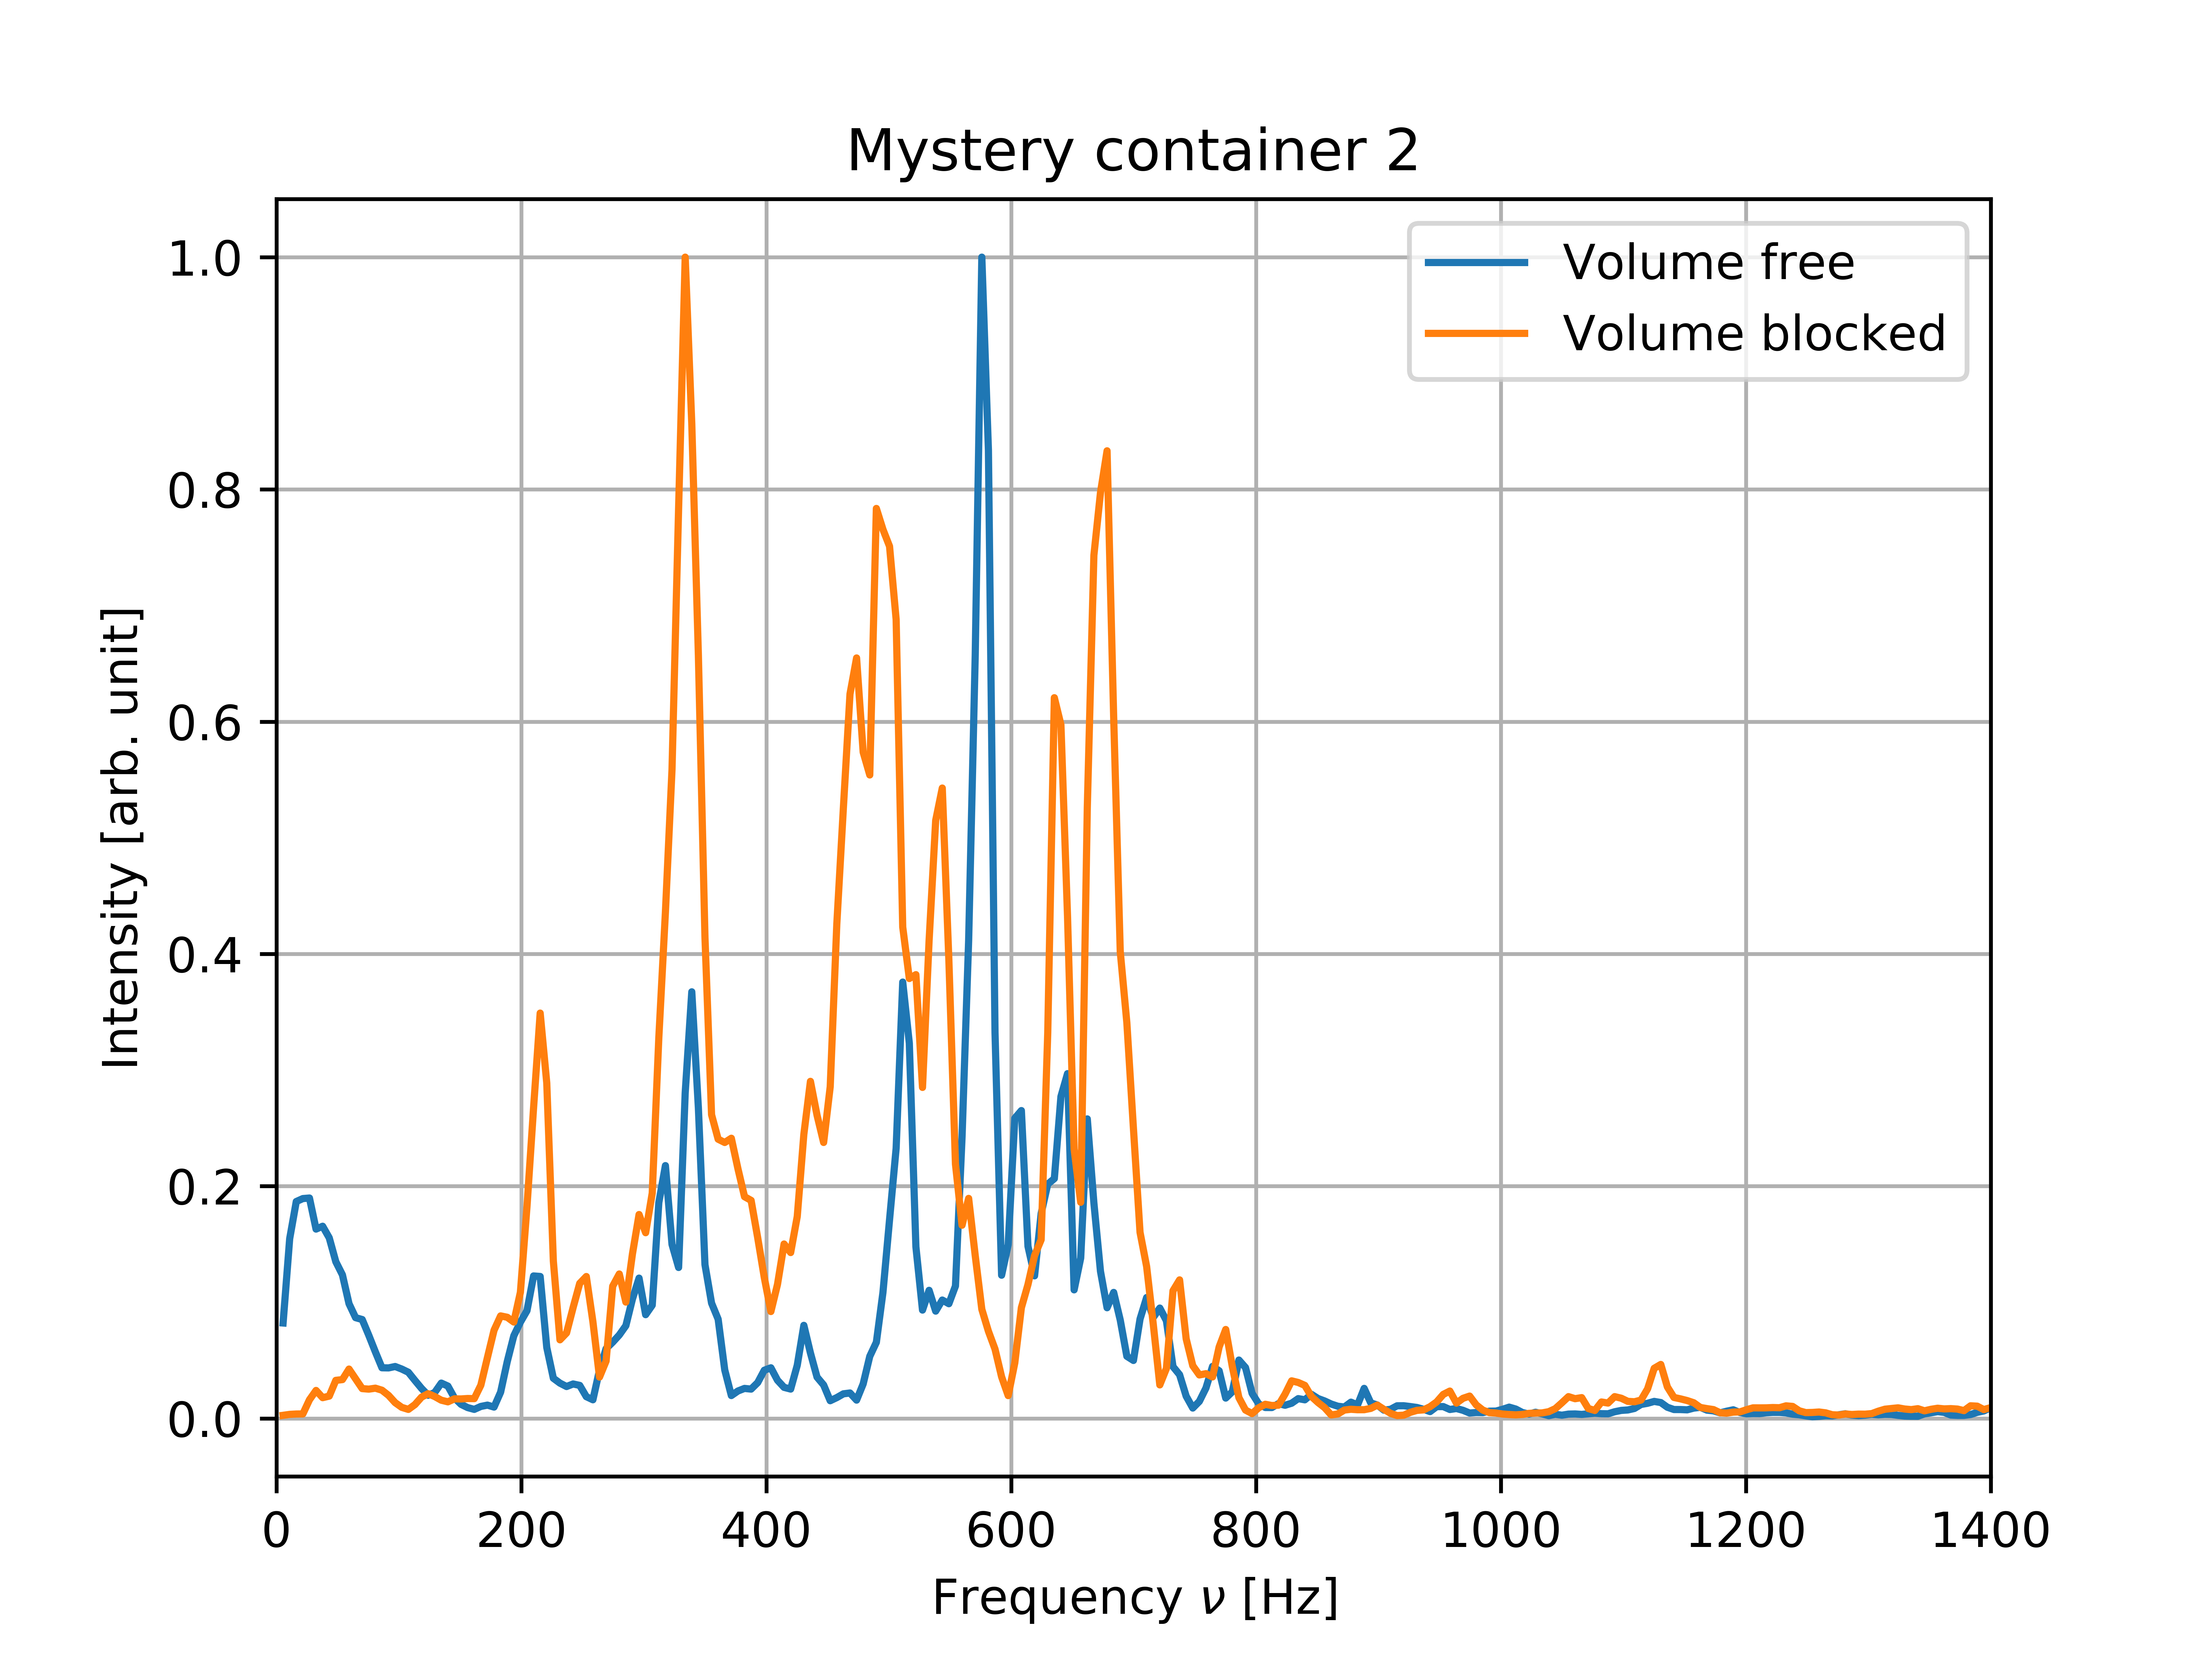
\includegraphics[scale=0.0305]{mystery3peaks.png}
\caption{Plot of the spectrum of mystery box 2.}
\label{mys3peaks}
\end{figure}

The spectra gotten from the mystery boxes didn't have any prominent features above $1400 \, \mathrm{Hz}$. This is partly because higher harmonics weren't excited but it also implies that the size of the containers is somewhat bigger than the tea box for example.

The overlap between blocked and free volume oscillation spectra is particularly high for mystery box 1. At first we thought that the most prominent peak was the one at $371 \, \mathrm{Hz}$. Together with the assumptions that the peak came from oscillations of a linear open dimension (most common for everyday containers) this frequency would give the size as $L \approx 23.1 \, \mathrm{cm}$. After the geometrically measured sizes of $L_x = 6.2 \, \mathrm{cm}$, $L_y = 8.3 \, \mathrm{cm}$ and $L_z = 8.1 \, \mathrm{cm}$ were revealed it was noticed that a better choice for the peak would have been $866 \, \mathrm{Hz}$, because it's the only one not covered by an orange peak at all. Calculations with that frequency give the size $L \approx 9.9 \, \mathrm{cm}$ which is a better fit. This actualizes the fact that reading off the peaks from the graph can sometimes be hard to do even with the help of oscillations with the volume blocked.

For mystery box 2 we have a somewhat better situation where at least one peak is definitely prominent enough, namely the one at $576 \, \mathrm{Hz}$. With the same assumptions as before of the dimension being linear and open we get $L \approx 14.9 \, \mathrm{cm}$. The actual measured sizes of mystery box 2 were $L_x = 8.7 \, \mathrm{cm}$, $L_y = 6.0 \, \mathrm{cm}$ and $L_z = 11.6 \, \mathrm{cm}$.

Considering that we can't find the end corrections because we don't know the other dimensions from the spectra, these turn out to be good approximations for the vertical sizes of the containers.


\section{Conclusions and Discussion}

Even though the mathematical question of recognizing shapes from their spectra has a clear answer, namely that they can mostly be distinguished, the physics question runs into additional complications. Theoretically, the problem of the inadequacy of the Neumann boundary condition for an open end gives rise to end corrections. While experimentally we are limited to only a window of the whole spectrum because of noise and microphone sensitivity.

But even with these restrictions some information can be extracted from the spectra of objects. Usually the geometry can't be determined because of the lack of higher harmonics which would have different distributions for different geometries. It is usual to be able to determine at least the largest of the dimensions under some assumptions on the geometry, such as that the largest dimension is linear and open (the most common case for everyday containers).

Theoretical improvements on the experiment would include a better formula for the end corrections or completely dispensing with them and introducing a more general formula for object with one open side.

Experimental improvements could include getting a better range of frequencies by trying to reduce noise and using a microphone with a larger span, and finding a better way to compare the intensities of the blocked and free oscillations so as to make recognizing free peaks easier.

\printbibliography

\end{document}